\section{State of the Art}
TODO
\subsection{TODO some papers}

\section{Interaction Diagrams}
\section{Scenario Testing}
Scenario testing, was originally introduced in \textcite{kaner2003power} and later as \textcite{kaner2013introduction}. The author defines scenarios as hypothetical stories, which aid a person in understanding a complex system or problem. Scenario tests are tests, which are based on such scenarios.  \parencite[1]{kaner2013introduction}
Further, \parencite[2-5]{kaner2003power} defines five characteristics, which make up a good scenario test as follows:
A Scenario test must be
\begin{itemize}
     \item based on a story - based on a description of how the program is being used
    \item motivating - stakeholders have interest in this test succeeding and would see to it's resolution
    \item credible - probable to happen in the real world
    \item complex - complex use, data or environment
    \item easy to evaluate - it should be easy to tell if the test succeded or failed based on the results 
\end{itemize}

\textcite{kaner2013introduction} describes the biggest advantages of scenario testing to be  - understanding and learning the product in early stages of development(1), connecting of testing and requirement documentations(2), exposing shortcomings in delivering of desired benefits(3), exploration of expert use of the program(4), expose requirement related issues(5).

\section{Behavior-Driven Development}
Behavior-Driven Development (BDD), pioneered by  \textcite{north2006behavior} is a software development
process , that combines principles from Test-Driven Development and Domain-Driven design \parencite{evans2004domain}.

Its main goal is to specify a system in terms of its functionality (i.e. it's behaviors) with a simple domain-specific language (DSL) making use of English-like sentences. This stimulates collaboration between developers and non-technical stakeholders and further results in a closer connection between acceptance criteria for a given function and matching tests used for its validation.

BDD splits a user story into multiple scenarios, each formulated in the form of \textit{Given}, \textit{When}, \textit{Then} statements, respectively specifying the prerequisite/context, event and outcomes of a scenario. 

[TODO] example here

At present ... there based on the division of behavior descriptions and behaviors. Such as Jest/Jasmine combine behavior descriptions and behaviors into one, whereas as Cucumber uses a DSL named Gherkin to specify the behavior descriptions and provides a set of tools to generate behaviors.
%[TODO example A vs B? ]


 \subsection{the other one(forgot name)}
 splitting into ...
\subsection{Gherkin Language}
\section{Vue.js}
structure etc.
template part
code part
bindings


\section{ESLint}

ESLint \parencite{eslintMainPage} is a linting tool (linter) for ECMAScript/JavaScript. Linters are static code analysis tool, which can be used to flag and potentially automatically fix common code issues and enforce consistent code styling.


\subsection{Architecture}

At a very high level, ESLint consists of 
\begin{figure}[H]
    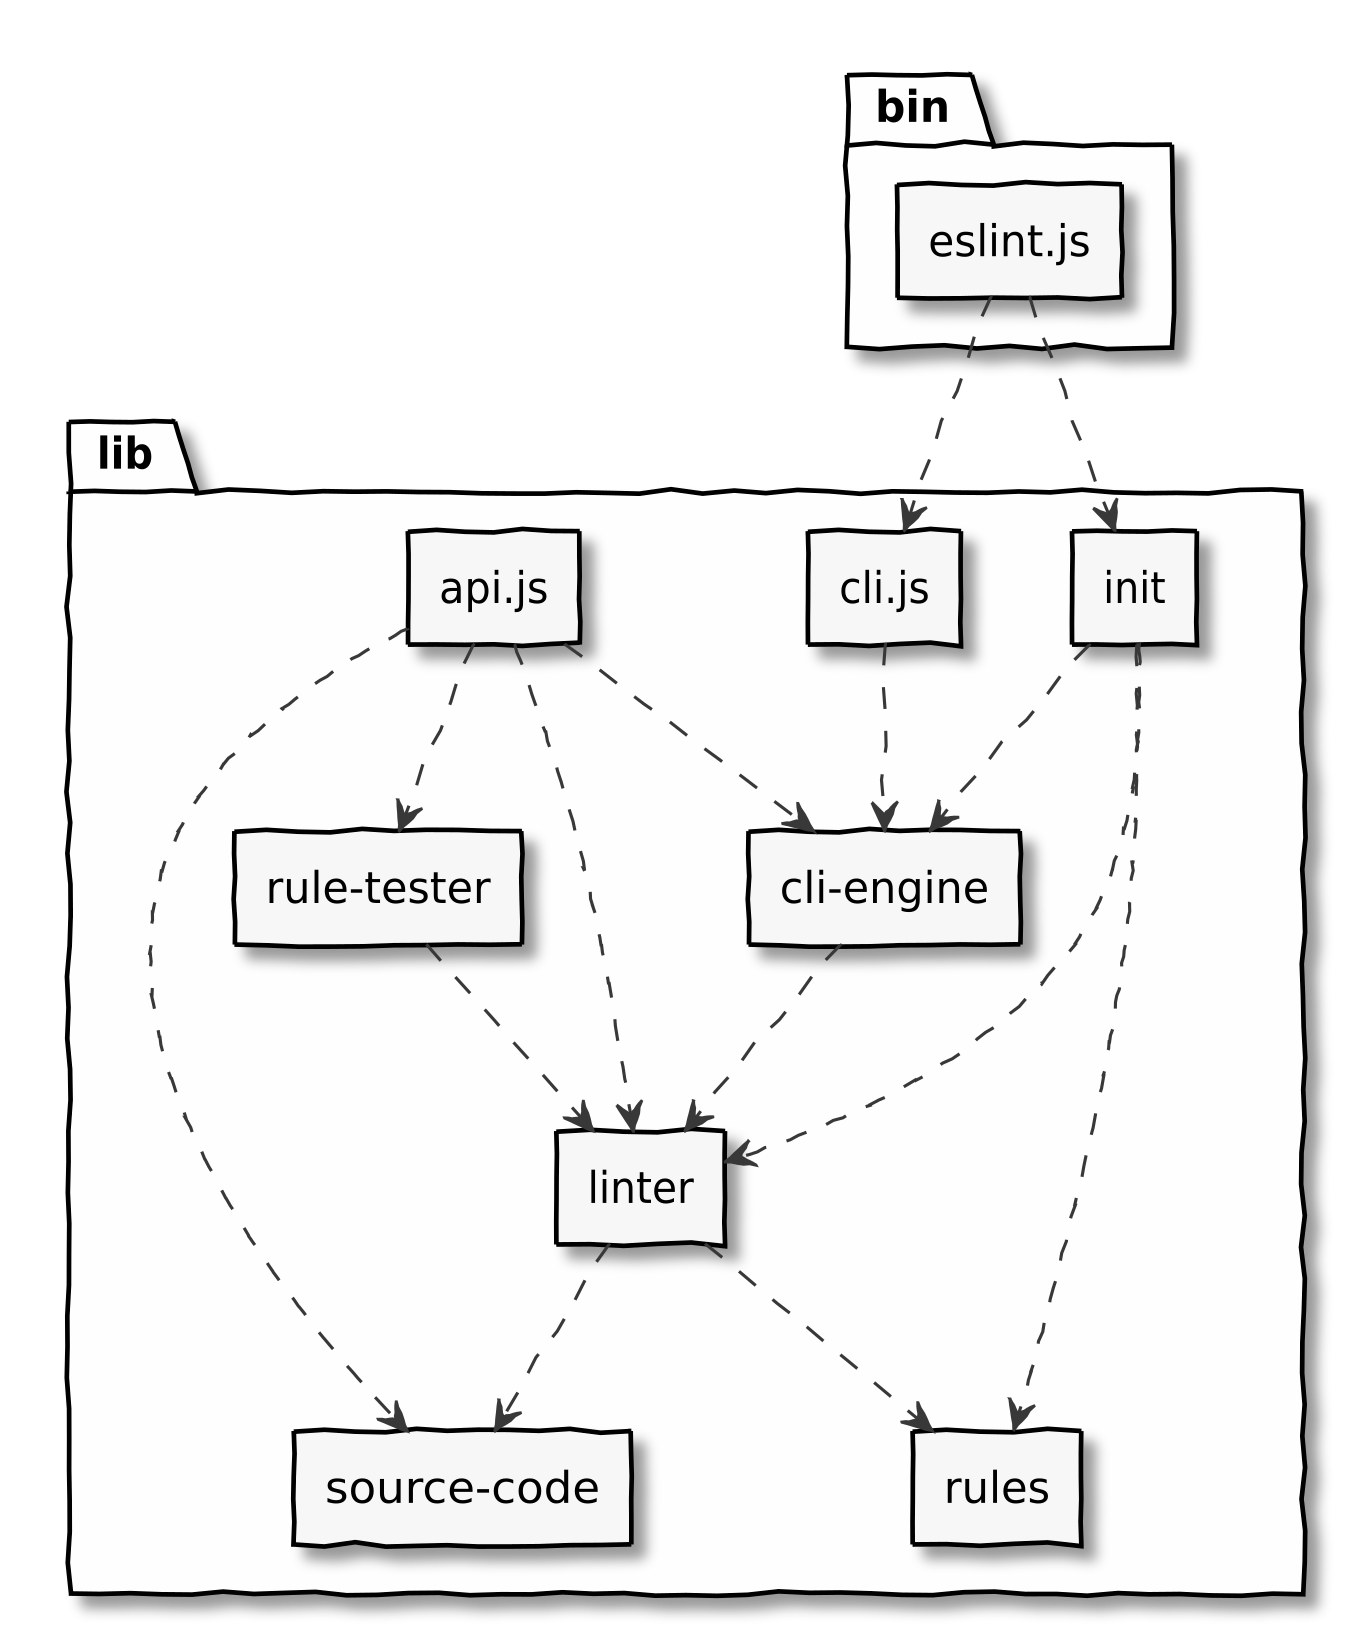
\includegraphics[width=\textwidth]{images/eslint_architecture.png}
     \caption{ESLint Architecture taken from \cite{eslintArchitecture}}
     \label{fig:eslintArchitecture}
   \end{figure}


\section{Rules}
At the core of ESLint are rules. Rules are extensible pieces of code, bundled as plugins, which can be used to verify various aspects of code. An example would be a rule, which checks for matching closing paranthesis. 
Each rule consists of a \code{metadata} object
and a \code{create} function. The metadata object includes metadata such as documentation strings, the type of the rule and whehter it is fixable or not.

Based on type, rules can be either \textit{suggestions}, \textit{problems} or \textit{layout}. Suggestions indicate some improvement, but are not required and would not cause the linting to fail. Problems on the other hand would result in a linting failure. Layouts are rules that care mainly about the formatting of code, such as whitespaces, semicolons, etc. 

If the fixable property is specified, it indicates that the errors reported by this rule can be automatically fixed. This can be applied via the \code{--fix} command line option. It has two possible values - \textit{code} or \textit{whitespace} indicating the type of fixes, that this rule would apply. For example in \glspl{ide} fixable \textit{code} errors would show a fix shortcut displayed next to them and \textit{whitespace} rules could be applied when saving the file.

The \code{create} function of rules takes as arguments a \code{context} and returns an object of methods which are called by ESLint for each node based on the \gls{visitor} pattern while traversing the \gls{ast}. ESLint provides a very powerful matching mechanism for specifying what nodes to match called selectors \parencite{eslintSelectors} inspired by \textcite{estoolsEsQuery}. 


TODO what are selectors

TODO what does context provide?

\subsection{AST Explorer}
An incredibly useful tool when working with \glspl{ast} is \gls{ast} Explorer, developed by \textcite{astexplorer_fkling2021Jan}. It enables the exploration of syntax tree generated by various parsers and also includes the vue-eslint-parser \parencite{eslint_vue_parser}

\subsection{ESTree AST}
By default ESLint uses the \parencite{eslintEspree} parser to parse JavaScript source code into an \gls{ast} as defined by ESTree specification \parencite{estreeASTSpec}. When Parsing \textit{.vue} files ESLint uses this parser for the code inside the \code{<script>} tag.
  
\subsection{ESLint Parser Vue AST}
In order to parse the \code{<template>} section of \textit{.vue} files, ESLint uses the vue-eslint-parser \parencite{eslint_vue_parser}. This parser outputs an  \gls{ast} compliant with their own  \gls{ast}specification, defined in \parencite{eslint_vue_parser_ast}.
